\documentclass{article}
\usepackage[utf8]{inputenc}
\usepackage{xcolor}
\usepackage{amsmath}
\usepackage{scrextend}
\usepackage{listings}
\usepackage{tcolorbox}
\usepackage{graphicx}
\usepackage{tikz}
\usepackage{float}
\usepackage{hyperref}
\usepackage[framemethod=tikz]{mdframed}

\setlength{\parindent}{0pt}
\setlength{\parskip}{12pt}
\setlength{\intextsep}{0pt plus 2pt}

% For setting margins
\usepackage[margin=2in]{geometry}


\definecolor{codeColor}{HTML}{282c34}
\definecolor{keyWord}{HTML}{0000ff}
\definecolor{variable}{HTML}{ffffff}
\definecolor{CommentColor}{HTML}{aaaaaa}
\definecolor{StrColor}{HTML}{00ff00}
\definecolor{ruleColor}{HTML}{282c34}

\graphicspath{{.}}

\lstset{backgroundcolor=\color{codeColor}, 
basicstyle=\fontfamily{pcr}\selectfont\footnotesize\color{variable},
commentstyle=\color{CommentColor},
stringstyle=\color{StrColor},
breaklines=true, 
rulecolor=\color{codeColor}}

\title{Assignment 3}
\date{}
\author{Jonas Valfridsson\\199608275377}

\begin{document}

\maketitle
\tableofcontents




All the code can be found at \href{https://github.com/DD2360-Assignments-Jonas-Valfridsson/Assignments}{https://github.com/DD2360-Assignments-Jonas-Valfridsson/Assignments}

\newpage  


\section{Exercise (1)}%

\subsection{Performance without shared memory}%
\label{ssub:performance_of_shared_memory}



On my 1080GTX-TI the execution time is:

\begin{center}
  \begin{tabular}{ | c | c | c | c | }
    \hline
    & hk.bmp & nyc.bmp & rome.bmp\\ \hline
    gray-scale-gpu & 13ms & 23ms & 8ms\\ \hline
    gray-scale-cpu & 55ms & 101ms & 34ms\\ \hline
    gaussian-gpu & 13ms & 23ms & 8ms\\ \hline
    gaussian-cpu & 380ms & 688ms & 234ms \\ \hline
    sobel-gpu & 13ms & 23ms & 8ms \\  \hline
    sobel-cpu & 792ms & 1434ms & 468ms \\  \hline
    \hline
  \end{tabular}
\end{center}

Here are some more detailed stats for the NYC.bmp

\begin{mdframed}[backgroundcolor=codeColor,leftmargin=0.0cm,hidealllines=true,%
  innerleftmargin=0.1cm,innerrightmargin=0.1cm,innertopmargin=0.5cm,innerbottommargin=0.10cm,
  roundcorner=15pt]
  \begin{lstlisting}[language=bash]
  ==26458== Profiling application: ./hw3_ex1 images/nyc.bmp
  ==26458== Profiling result:
  Time(%)      Time     Calls       Avg  Name
  44.29%  44.107ms         1  44.107ms  [CUDA memcpy HtoD]
  37.71%  37.547ms         3  12.516ms  [CUDA memcpy DtoH]
  7.96%  7.9257ms         1  7.9257ms  gpu_grayscale(int, ..)
  7.92%  7.8828ms         1  7.8828ms  gpu_gaussian(int, ..)
  2.12%  2.1115ms         1  2.1115ms  gpu_sobel(int, ..)
  0.00%  3.5840us         2  1.7920us  [CUDA memset]
  53.89%  123.09ms         3  41.030ms  cudaMalloc
  45.02%  102.84ms         4  25.709ms  cudaMemcpy
  0.64%  1.4540ms         3  484.66us  cudaFree
  0.22%  501.57us         1  501.57us  cuDeviceTotalMem
  0.15%  336.92us        96  3.5090us  cuDeviceGetAttribute
  0.04%  92.333us         3  30.777us  cudaLaunchKernel
  0.02%  35.764us         1  35.764us  cuDeviceGetName
  0.01%  30.695us         2  15.347us  cudaMemset
  0.01%  14.635us         1  14.635us  cuDeviceGetPCIBusId
  0.00%  6.5460us         2  3.2730us  cuDeviceGet
  0.00%  1.9270us         3     642ns  cuDeviceGetCount
  0.00%     384ns         1     384ns  cuDeviceGetUuid
  \end{lstlisting}
\end{mdframed}


\subsection{Mapping of GPU threads and thread-blocks}%
\label{sub:mapping_of_gpu_threads_and_thread_blocks}

We have a 2D image that is flattened to a 2D array such that we get the index function $f: (x, y) \rightarrow x + W * y$ where W is the image width. Our GPU threads 
and blocks are also stored as 2D structures - we can calculate the y index in our 2D image of our GPU topology by using the threadIdx.y, blockIdx.y blockDim.y

$$ y= threadIdx.y + blockIdx.y * blockDim.y$$ 

And the same for x

$$ x = threadIdx.x + blockIdx.x * blockDim.x $$ 

Then we can use the index function (f) to index into our flattened image. Essentially each GPU thread block is responsible for a tiny block on the original image.

\subsection{Why shared memory can improve performance}%
\label{sub:why_shared_memory_can_improve_performance}

Shared memory is located on the SM - it is much smaller than global memory but has much faster reads. So in the case when we are doing convolutions we are accessing each
pixel multiple times. In cases like this it might be worth to read it from global memory and then store it in shared the first time, so that subsequent memory accesses is much faster. On 
Nvidias Website it says that shared memory access can be up to 100x faster than global memory - This can lead to large performance gains when a thread block accesses the same memory multiple times.

\subsection{Why we get black squares}%

The reason is because our shared memory is padded so that the thread block has access to all the data it need to perform the convolution. When each thread only loads its responsible pixel it does not also load in 
the value for the padding - this makes the shared memory 0 padded and gives these black boxes. So we also have to load in the padding into the shared memory - This can be seen in my code by the extra code-blocks that
checks if pixels are on the boundary, and if they are: loads in additional pixels.

\subsection{Performance With Shared Memory}%
\label{sub:}

File sizes are: hk.bmp is 38MB nyc.bmp is 69MB and rome.bmp is 24MB


\begin{center}
  \begin{tabular}{ | c | c | c | c | }
    \hline
    & hk.bmp & nyc.bmp & rome.bmp\\ \hline
    gray-scale-gpu & 13ms & 23ms & 8ms\\ \hline
    gray-scale-cpu & 55ms & 101ms & 34ms\\ \hline
    gaussian-gpu & 13ms & 23ms & 8ms\\ \hline
    gaussian-cpu & 380ms & 688ms & 234ms \\ \hline
    sobel-gpu & 13ms & 23ms & 8ms \\  \hline
    sobel-cpu & 792ms & 1434ms & 468ms \\  \hline
    \hline
  \end{tabular}
\end{center}

Here are some more detailed stats for the NYC.bmp

\begin{mdframed}[backgroundcolor=codeColor,leftmargin=0.0cm,hidealllines=true,%
  innerleftmargin=0.1cm,innerrightmargin=0.1cm,innertopmargin=0.5cm,innerbottommargin=0.10cm,
  roundcorner=15pt]
  \begin{lstlisting}[language=bash]
  ==2163== Profiling application: ./hw3_ex1 images/nyc.bmp
  ==2163== Profiling result:
  Time(%)      Time     Calls       Avg  Name
  39.27%  44.065ms         1  44.065ms  [CUDA memcpy HtoD]
  38.87%  43.616ms         3  14.539ms  [CUDA memcpy DtoH]
  7.64%  8.5695ms         1  8.5695ms  gpu_sobel(int, ...)
  7.15%  8.0183ms         1  8.0183ms  gpu_gaussian(int, ...)
  7.06%  7.9265ms         1  7.9265ms  gpu_grayscale(int, ...)
  0.00%  3.6800us         2  1.8400us  [CUDA memset]
  50.79%  123.32ms         3  41.107ms  cudaMalloc
  47.58%  115.52ms         4  28.879ms  cudaMemcpy
  1.37%  3.3220ms         3  1.1073ms  cudaFree
  0.09%  230.25us        96  2.3980us  cuDeviceGetAttribute
  0.09%  221.73us         1  221.73us  cuDeviceTotalMem
  0.05%  123.82us         3  41.272us  cudaLaunchKernel
  0.01%  35.951us         2  17.975us  cudaMemset
  0.01%  17.451us         1  17.451us  cuDeviceGetName
  0.00%  7.3310us         1  7.3310us  cuDeviceGetPCIBusId
  0.00%     896ns         3     298ns  cuDeviceGetCount
  0.00%     710ns         2     355ns  cuDeviceGet
  0.00%     167ns         1     167ns  cuDeviceGetUuid
  \end{lstlisting}
\end{mdframed}


I see essentially no difference between shared memory here and not shared memory. But there is a good explanation for it. When I started implementing shared memory and had the black square issues, my Rome solution was 1ms
faster (it was 7ms). But when I added all of the additional bounds-checking to load in all the correct data it got slower again. So there is this trade-off between how much work needs to be done to load the correct data into
shared memory vs the gains of using it. Perhaps my loading code can be made more efficient, in that case I'd see gains - so the lesson learned is that shared memory is great if I need to operate on some memory multiple times
across threads in a thread block.

\section{Exercise (2)}%
\label{sec:exercise_2_}


With unpinned memory 

\begin{mdframed}[backgroundcolor=codeColor,leftmargin=0.0cm,hidealllines=true,%
  innerleftmargin=0.1cm,innerrightmargin=0.1cm,innertopmargin=0.5cm,innerbottommargin=0.10cm,
  roundcorner=15pt]
  \begin{lstlisting}[language=bash]
  ==13944== Profiling ..: ./exercise_2 10000000 100 64
  ==13944== Profiling result:
  Time(%)      Time     Calls       Avg  Name
  43.77%  2.66025s       100  26.602ms  [CUDA memcpy DtoH]
  43.06%  2.61738s       100  26.174ms  [CUDA memcpy HtoD]
  13.17%  800.26ms       100  8.0026ms  gpu_step(int, ..)
  98.02%  6.09644s       200  30.482ms  cudaMemcpy
  1.96%  121.80ms         1  121.80ms  cudaMalloc
  0.01%  881.49us       100  8.8140us  cudaLaunchKernel
  0.00%  297.28us         1  297.28us  cudaFree
  0.00%  223.55us        96  2.3280us  cuDeviceGetAttribute
  0.00%  222.47us         1  222.47us  cuDeviceTotalMem
  0.00%  17.776us         1  17.776us  cuDeviceGetName
  0.00%  7.7810us         1  7.7810us  cuDeviceGetPCIBusId
  0.00%  3.3900us         1  3.3900us  cudaDeviceSynchronize
  0.00%  3.3850us         2  1.6920us  cuDeviceGet
  0.00%     849ns         3     283ns  cuDeviceGetCount
  0.00%     165ns         1     165ns  cuDeviceGetUuid
  \end{lstlisting}
\end{mdframed}

\newpage 

With pinned memory
\begin{mdframed}[backgroundcolor=codeColor,leftmargin=0.0cm,hidealllines=true,%
  innerleftmargin=0.1cm,innerrightmargin=0.1cm,innertopmargin=0.5cm,innerbottommargin=0.10cm,
  roundcorner=15pt]
  \begin{lstlisting}[language=bash]
  ==17937== Profiling ..: ./exercise_2 10000000 100 64
  ==17937== Profiling result:
  Time(%)      Time     Calls       Avg  Name
  42.08%  2.12402s       100  21.240ms  [CUDA memcpy HtoD]
  41.81%  2.11049s       100  21.105ms  [CUDA memcpy DtoH]
  16.11%  813.29ms       100  8.1329ms  gpu_step(int, ..)
  96.89%  5.05152s       200  25.258ms  cudaMemcpy
  3.08%  160.38ms         1  160.38ms  cudaHostAlloc
  0.01%  531.10us       100  5.3110us  cudaLaunchKernel
  0.01%  490.40us         1  490.40us  cudaMalloc
  0.01%  328.79us         1  328.79us  cudaFree
  0.01%  260.93us         1  260.93us  cuDeviceTotalMem
  0.00%  229.47us        96  2.3900us  cuDeviceGetAttribute
  0.00%  18.750us         1  18.750us  cuDeviceGetName
  0.00%  7.2260us         1  7.2260us  cuDeviceGetPCIBusId
  0.00%  3.1610us         1  3.1610us  cudaDeviceSynchronize
  0.00%     861ns         2     430ns  cuDeviceGet
  0.00%     813ns         3     271ns  cuDeviceGetCount
  0.00%     164ns         1     164ns  cuDeviceGetUuid
  \end{lstlisting}
\end{mdframed}


Using pinned memory vs unpinned memory made the whole program 17\% faster for 1e7 particles over 100 steps.


\newpage

With managed-memory
\begin{mdframed}[backgroundcolor=codeColor,leftmargin=0.0cm,hidealllines=true,%
  innerleftmargin=0.1cm,innerrightmargin=0.1cm,innertopmargin=0.5cm,innerbottommargin=0.10cm,
  roundcorner=15pt]
  \begin{lstlisting}[language=bash]
  ==20413== Profiling ..: ./exercise_2b 10000000 100 64
  ==20413== Profiling result:
  Time(%)      Time     Calls       Avg Name
  100.00%  303.82ms       100  3.0382ms gpu_step(int, ..)
  63.97%  303.54ms         1  303.54ms cudaDeviceSynchronize
  30.14%  143.02ms         1  143.02ms cudaMallocManaged
  3.67%  17.424ms       100  174.24us cudaLaunchKernel
  2.06%  9.7601ms         1  9.7601ms cudaFree
  0.08%  402.42us         1  402.42us cuDeviceTotalMem
  0.06%  295.20us        96  3.0740us cuDeviceGetAttribute
  0.01%  32.112us         1  32.112us cuDeviceGetName
  0.00%  14.112us         1  14.112us cuDeviceGetPCIBusId
  0.00%  5.6590us         2  2.8290us cuDeviceGet
  0.00%  1.6650us         3     555ns cuDeviceGetCount
  0.00%     334ns         1     334ns cuDeviceGetUuid

  ==20413== Unified Memory profiling result:
  Device "GeForce GTX 1080 Ti (0)"
  Count  Avg Size Total Size  Total Time  Name
  5387  35.190KB 185.1289MB  18.68624ms  Host To Device
  1376  170.28KB 228.8203MB  19.11085ms  Device To Host
  356         -          -  41.64218ms  Gpu page fault ..
  Total CPU Page faults: 1378
  \end{lstlisting}
\end{mdframed}

Managed memory appears significantly faster, but I am not doing any actual copies in the inner loop with it. What if we read the managed memory on the CPU inside the loop in each iteration?

\newpage

\begin{mdframed}[backgroundcolor=codeColor,leftmargin=0.0cm,hidealllines=true,%
  innerleftmargin=0.1cm,innerrightmargin=0.1cm,innertopmargin=0.5cm,innerbottommargin=0.10cm,
  roundcorner=15pt]
  \begin{lstlisting}[language=bash]
  ==20996== Profiling application: ./exercise_2b 10000000 100 64
  ==20996== Profiling result:
  Time(%)      Time     Calls       Avg Name
  100.00%  6.03312s       100  60.331ms gpu_step(int, ..)
  88.10%  143.43ms         1  143.43ms cudaMallocManaged
  5.17%  8.4103ms         1  8.4103ms cudaDeviceSynchronize
  4.30%  6.9965ms         1  6.9965ms cudaFree
  1.97%  3.2093ms       100  32.093us cudaLaunchKernel
  0.25%  402.13us         1  402.13us cuDeviceTotalMem
  0.18%  299.91us        96  3.1240us cuDeviceGetAttribute
  0.02%  31.252us         1  31.252us cuDeviceGetName
  0.01%  14.486us         1  14.486us cuDeviceGetPCIBusId
  0.00%  2.6220us         3     874ns cuDeviceGetCount
  0.00%  1.1110us         2     555ns cuDeviceGet
  0.00%     327ns         1     327ns cuDeviceGetUuid

  ==20996== Unified Memory profiling result:
  Device "GeForce GTX 1080 Ti (0)"
  Count  Avg Size   Total Size  Total Time  Name
  524270  38.060KB   19.02934GB   2.280476s  Host To Device
  120118  164.17KB   18.80582GB   1.885460s  Device To Host
  42837         -            -   5.648922s  Gpu page fault ..
  355         -            -  227.8919ms  Page throttles
  3762  4.0000KB   14.69531MB           -  Memory thrashes
  Total CPU Page faults: 61759
  Total CPU thrashes: 3762
  Total CPU throttles: 34
  \end{lstlisting}
\end{mdframed}

What if we write to it in each iteration?

\newpage 

\begin{mdframed}[backgroundcolor=codeColor,leftmargin=0.0cm,hidealllines=true,%
  innerleftmargin=0.1cm,innerrightmargin=0.1cm,innertopmargin=0.5cm,innerbottommargin=0.10cm,
  roundcorner=15pt]
  \begin{lstlisting}[language=bash]
  ==21095== Profiling application: ./exercise_2b 10000000 100 64
  ==21095== Profiling result:
  Time(%)      Time     Calls       Avg  Name
  100.00%  5.50782s       100  55.078ms  gpu_step(int, ...)
  91.37%  145.94ms         1  145.94ms  cudaMallocManaged
  6.25%  9.9809ms         1  9.9809ms  cudaFree
  2.06%  3.2922ms       100  32.922us  cudaLaunchKernel
  0.15%  236.62us         1  236.62us  cuDeviceTotalMem
  0.14%  226.66us        96  2.3610us  cuDeviceGetAttribute
  0.02%  33.053us         1  33.053us  cuDeviceGetName
  0.01%  11.982us         1  11.982us  cudaDeviceSynchronize
  0.00%  7.2890us         1  7.2890us  cuDeviceGetPCIBusId
  0.00%     929ns         3     309ns  cuDeviceGetCount
  0.00%     575ns         2     287ns  cuDeviceGet
  0.00%     162ns         1     162ns  cuDeviceGetUuid

  ==21095== Unified Memory profiling result:
  Device "GeForce GTX 1080 Ti (0)"
  Count  Avg Size Total Size  Total Time  Name
  473566  38.175KB 17.24089GB   2.060307s  Host To Device
  110407  163.73KB 17.23896GB   1.725519s  Device To Host
  39222         -          -   5.069925s  Gpu page fault ...
  311         -          -  159.9216ms  Page throttles
  3554  4.0000KB 13.88281MB           -  Memory thrashes
  Total CPU Page faults: 57047
  Total CPU thrashes: 3554
  Total CPU throttles: 27

  \end{lstlisting}
\end{mdframed}

In summary, pinned memory was 17\% faster than unpinned memory in my benchmark, managed memory was 2.2x faster than pinned memory when I don't actually read or write to it on the CPU. If i read or write to it on CPU in the loop then managed
memory was 40\% slower than unpinned memory. Here's a graph to summarize the results:


\begin{figure}[H]
  \centering
  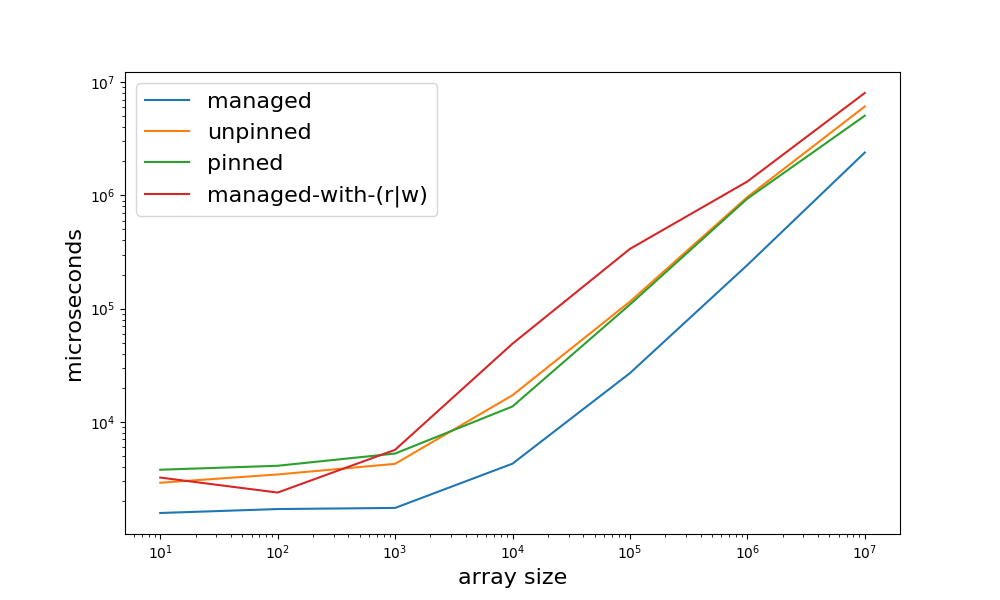
\includegraphics[width=0.98\linewidth]{ex_2/simulation-time.png}
  \label{fig:}
\end{figure}

\subsection{Trade-Offs Pageable vs Pinned}%
\label{sub:trade_offs_pageable_vs_pinned}

Pinning yields faster host-to-device and device-to-host copies. The reason for this is because the GPU has to pin the memory either way to transfer it to the device, it cannot copy from pageable memory.  a problem with
manually pinning memory on the host is that you are occupying a chunck of physical RAM on the host - RAM that could potentially have been better used if it was pageable. Also pinning memory takes time, it is slower than
malloc so it should not be done excessively.

\subsection{Pinned Memory Performance Improvement}%
\label{sub:trade_offs_pageable_vs_pinned}

Yes - by pinning the memory I got a 17\% performance improvement on the total runtime of the program - it went from taking 60ms to 50ms. Both the H2D and D2H got about 5ms faster each.

\subsection{What is managed memory?}%
\label{sub:what_is_managed_memory_}



Managed memory makes use of a unified memory address space that is accessible from both the host and the device. It is a smart way to let cuda handle more of the memory management and let the programmer focus more on the
algorithm. There are still things to consider though to maximize performance, such as prefetching memory onto the GPU.

\subsection{On tegner a implicit copy happends, why?}%
\label{sub:on_tegner_a_implicit_copy_happends_why_}



Managed memory works differently under the hood on different GPU archs - I guess tegner uses pascal or later: For these architechtures memory might not be physically allocated on the GPU when managedMemory is allocated. The
memory will be allocated when it is used (unless it is prefetched). Therefore the first kernel launch is the first to use the managed memory and that is when it is allocated, if running on a later arch.

\section{Exercise (3)}%
\label{sec:exercise_3_}

In my implementation the batch-size is determined by the number of streams, we can vary the batch-size by varying the number of streams.


\begin{figure}[H]
  \centering
  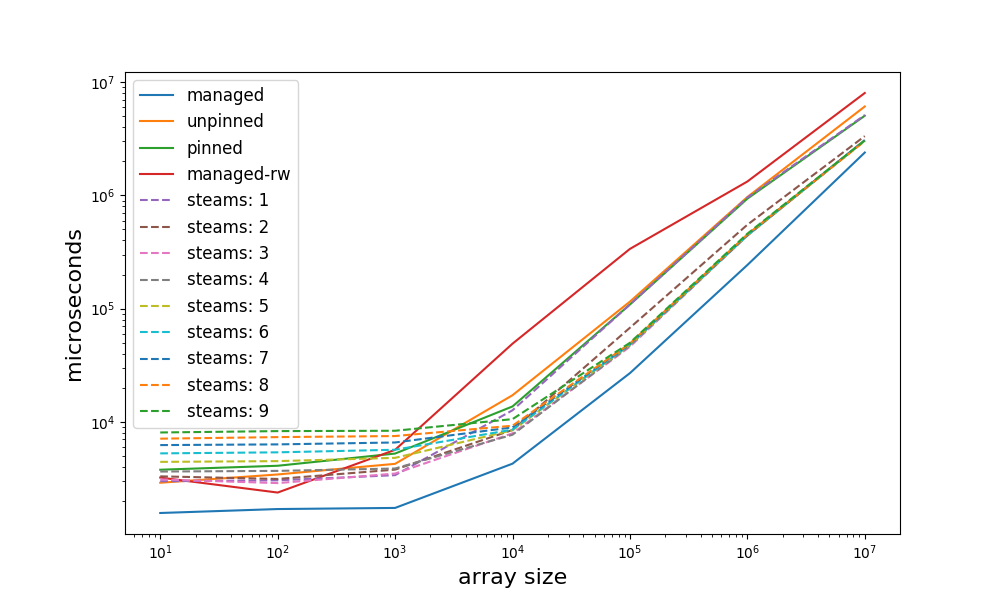
\includegraphics[width=0.98\linewidth]{ex_3/simulation-time.png}
  \label{fig:}
\end{figure}

As we can see the biggest gain is when we go from 1 streams to two streams, two streams to more streams give less gains. Using streams gave an impressive performance boost though - at 9 streams we have a performance boost of
1.7x almost as good as managed memory when we don't do any copies, very impressive! 

Here's the more detailed nvprof from when we use 9streams


\begin{mdframed}[backgroundcolor=codeColor,leftmargin=0.0cm,hidealllines=true,%
  innerleftmargin=0.1cm,innerrightmargin=0.1cm,innertopmargin=0.5cm,innerbottommargin=0.10cm,
  roundcorner=15pt]
  \begin{lstlisting}[language=bash]
  ==18856== Profiling ...: ./exercise_3 10000000 100 64 9
  ==18856== Profiling result:
  Time(%)      Time  Calls       Avg Name
  36.97%  3.05627s    900  3.3959ms [CUDA memcpy HtoD]
  35.70%  2.95184s    900  3.2798ms [CUDA memcpy DtoH]
  27.33%  2.25965s    900  2.5107ms gpu_step(int, ..)
  94.71%  3.05729s      1  3.05729s cudaDeviceSynchronize
  4.99%  161.13ms      1  161.13ms cudaHostAlloc
  0.14%  4.4937ms   1800  2.4960us cudaMemcpyAsync
  0.11%  3.5283ms    900  3.9200us cudaLaunchKernel
  0.01%  408.80us      1  408.80us cudaMalloc
  0.01%  391.59us      1  391.59us cuDeviceTotalMem
  0.01%  302.36us      2  151.18us cudaFree
  0.01%  298.45us      9  33.161us cudaStreamCreate
  0.01%  295.68us     96  3.0800us cuDeviceGetAttribute
  0.00%  30.718us      1  30.718us cuDeviceGetName
  0.00%  15.022us      1  15.022us cuDeviceGetPCIBusId
  0.00%  5.5610us      2  2.7800us cuDeviceGet
  0.00%  1.6360us      3     545ns cuDeviceGetCount
  0.00%     320ns      1     320ns cuDeviceGetUuid

  \end{lstlisting}
\end{mdframed}

And here's a snapshot of the visual profiler

\begin{figure}[H]
  \centering
  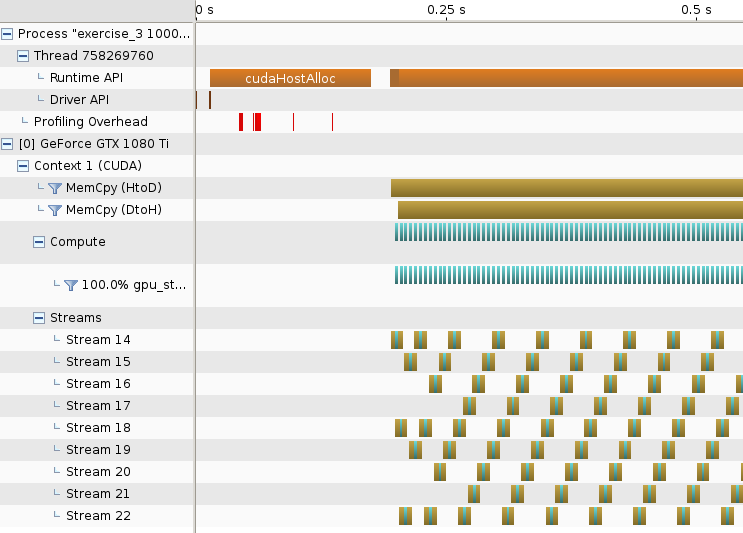
\includegraphics[width=0.98\linewidth]{ex_3/nvvprof.png}
  \label{fig:}
\end{figure}

It looks like the streams are executing concurrently in a nice staircase pattern.

\subsection{What are advantages of Streams?}%
\label{sub:what_are_advantages_of_streams_}

The streams lets us leverage concurrency to pipeline operations such that we maximize utilization of the GPU hardware - e.g when one stream is waiting for IO another stream can use more SM's to execute its kernel. 

\subsection{What is the performance improvement?}%
\label{sub:what_is_the_performance_improvement_}


I got a performance improvement of about 70\% over pinned memory when using streams, which is impressive!

\subsection{What is the impact of batch size?}%
\label{sub:what_is_the_impact_of_batch_size}


We want to have a batch size so that the GPU can spend as little time as possible on scheduling IO operations and at the same time never have to wait for IO operations. E.g too big of a batch size we will end up having to
wait for IO, too small of a batch-size will give us a lot of context switching and having to schedule IO which is just unnecessary operations. So we want to use a number of streams and a batch-size so that we can maximize
the relevant work we do on the GPU will minimizing the waiting time and unnecessary operations we have to do.


\section{cuBLAS}%
\label{sec:cublas}

result from my implementations: 


\begin{mdframed}[backgroundcolor=codeColor,leftmargin=0.0cm,hidealllines=true,%
  innerleftmargin=0.1cm,innerrightmargin=0.1cm,innertopmargin=0.5cm,innerbottommargin=0.10cm,
  roundcorner=15pt]
  \begin{lstlisting}[language=bash]
  ./exercise_3 -s 1024 -v

  Matrix size: 1024x1024
  Matrix size: 1024x1024
  Grid size: 64x64
  Tile size: 16x16
  Run CPU sgemm: 1

  CPU matmul:                     3663.794000 ms
  GPU matmul (global memory):     160.025000 ms
  GPU matmul (shared memory):     17.476000 ms
  GPU cuBLAS matmul:              2.834000 ms
  \end{lstlisting}
\end{mdframed}


\subsection{Why matrix size has to be multiple of 16?}%
\label{sub:why_matrix_size_has_t_obe_multiple_of_16}

This question is a lie! The matrix does not have to be a multiple of 16 if we change the tile size. The matrix have to be a multiple of the tile size
so that we can tile the matrix (subdivide it evenly into our tiles).

\subsection{Why two syncthreads?}%

The first syncthreads is to make sure the tile is completely updated before we start doing the sub-multiplication. The second sync is to avoid that the tile gets overwritten before the sub-multiplication is done.

\subsubsection{Directive to Improve}%
\label{ssub:directive_to_improve}

We can unroll the loop with a pragma

\subsubsection{Large speed-up}%
\label{ssub:large_speed_up}

Because we do TILE\_SIZE number of reads from the shared
memory and we don't have to do a lot of work to fill the
shared memory. The explanation is that we're better utilizing
it here.


\subsection{Why BA instead of AB?}%
\label{sub:why_ba_instead_of_ab_}
Because on our host we store the matrices in row-major order - but CUDA assumes they are in column major order. We can solve this by doing transpositions of our matrices and our result, or by just switching the order of multiplication.

\subsection{Different input sizes}%
\label{sub:different_input_sizes}



\begin{figure}[H]
  \centering
  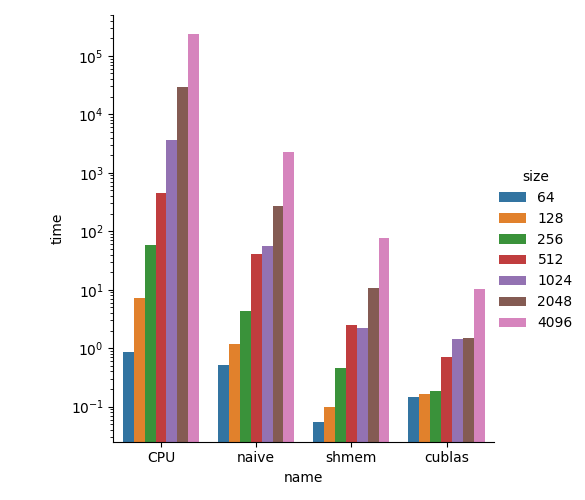
\includegraphics[width=0.98\linewidth]{ex_3/ex_bonus/simulation-time.png}
  \label{fig:}
\end{figure}

Notice that the y-scale is log-scale. Here we can see that for 4096 cublas is about 10000x faster than my CPU. That is insane.

\subsection{Benchmarking}%
\label{sub:benchmarking}

All code should be benchmarked with the same timer, also our timing include things such as context switching from the OS and all the surrounding things. We're not just benchmarking the GPU algorithm - but these other things
are negligible when our process takes a sufficient amount of time - Also we're including synchronization in our benchmark which might or might not be relevant for different applications.

\end{document}




